

% \begin{table*}[bh]
% \vspace{-0.8em}
% \caption{Performance on synthetic and real-world datasets with target confidence $1-\alpha = 0.9$ (for horizon $T=200$ for synthetic datasets, $300$ for electricity and traffic, and $60$ for bee, mean $\pm$ standard deviation of the test samples).  Methods that are \textit{invalid} (coverage below $90\%$) are grayed out. Our method achieves a high level of calibration (coverage is close to $90\%$) consistently. }
% \label{tab:baselines}
% \centering
% \resizebox{\textwidth}{!}{%
% \begin{tabular}{ l | c | c  c c c c c } 
% \toprule
% & & RED-SDS & CP & ACI & SPCI  & HopCPT & Ours \\ 
% \midrule\midrule
% \multirow{2}{*}{\begin{tabular}{l}Bouncing  \\ Ball obs.\end{tabular}} & Cov & \color{gray}{59.14 \plusminus 23.75}& \color{gray}{39.27 \plusminus 6.77}& \color{gray}{76.97 \plusminus 1.27}& \color{gray}{37.90 \plusminus 9.78}& \color{gray}{59.45 \plusminus 12.51} &91.03 \plusminus 1.37\\ 
%  & Width & \color{gray}{2.12 \plusminus 0.05}& \color{gray}{1.71 \plusminus 0.93}& \color{gray}{3.67 \plusminus 0.91}& \color{gray}{1.45 \plusminus 0.85}& \color{gray}{1.98 \plusminus 0.90} & 2.13 \plusminus 2.15\\ 
% \midrule
% \multirow{2}{*}{\begin{tabular}{l}Bouncing  \\ Ball dyn.\end{tabular}} & Cov & \color{gray}{43.46 \plusminus 27.18}& \color{gray}{40.41 \plusminus 6.89}& \color{gray}{76.63 \plusminus 0.95}& \color{gray}{53.62 \plusminus 7.75}& \color{gray}{61.12 \plusminus 4.80} &90.44 \plusminus 1.51\\ 
%  & Width & \color{gray}{1.80 \plusminus 0.03}& \color{gray}{0.89 \plusminus 0.45}& \color{gray}{2.97 \plusminus 1.07}& \color{gray}{2.02 \plusminus 0.23}& \color{gray}{2.95 \plusminus 1.12} & 4.92 \plusminus 2.79\\ 
% \midrule
% \multirow{2}{*}{\begin{tabular}{l}3-Mode \\ System\end{tabular}} & Cov & 92.98 \plusminus 3.01& \color{gray}{63.97 \plusminus 5.03}& \color{gray}{86.25 \plusminus 0.84}& \color{gray}{81.72 \plusminus 2.88}& 89.85 \plusminus 2.90 & 93.35 \plusminus 3.51\\ 
%  & Width & 2.08 \plusminus 0.16& \color{gray}{1.46 \plusminus 0.51}& \color{gray}{2.61 \plusminus 0.53}& \color{gray}{3.94 \plusminus 0.85}& 9.07 \plusminus 1.23 &  13.68 \plusminus 2.49\\ 
% \midrule
% \midrule
% \multirow{2}{*}{\begin{tabular}{l}Traffic\end{tabular}} & Cov & \color{gray}{86.55 \plusminus 11.20}& \color{gray}{69.64 \plusminus 2.62}& \color{gray}{88.19 \plusminus 0.33}& 88.24 \plusminus 2.13& 88.91 \plusminus 3.55 & 94.76 \plusminus 4.93\\ 
%  & Width & \color{gray}{2.81 \plusminus 1.54}& \color{gray}{0.32 \plusminus 0.22}& \color{gray}{56.92 \plusminus 25.26}& 4.62 \plusminus 2.28 & 7.50 \plusminus 10.09 & 8.34 \plusminus 14.44\\ 
% \midrule
% \multirow{2}{*}{\begin{tabular}{l}Electricity\end{tabular}} & Cov & \color{gray}{75.46 \plusminus 14.23}& \color{gray}{68.88 \plusminus 3.12}& \color{gray}{87.94 \plusminus 0.34}& \color{gray}{86.62 \plusminus 2.97} & \color{gray}{86.50 \plusminus 2.66} & 92.62 \plusminus 6.14\\ 
%  & Width & \color{gray}{87.47 \plusminus 119.95}& \color{gray}{58.62 \plusminus 456.89}& \color{gray}{28.28 \plusminus 169.33}& \color{gray}{371.69 \plusminus 305.86}& \color{gray}{155.71 \plusminus 130.43} & 166.88 \plusminus 129.07 \\ 
% \midrule
% \multirow{2}{*}{\begin{tabular}{l}Dancing \\ Bees\end{tabular}} & Cov & 90.79 \plusminus 5.03& \color{gray}{65.58 \plusminus 7.05}& \color{gray}{75.16 \plusminus 3.33}& \color{gray}{79.2 \plusminus 0.3} & \color{gray}{72.11 \plusminus 1.84} & 93.43 \plusminus 11.42 \\
%  & Width & 0.27 \plusminus 0.05& \color{gray}{0.12 \plusminus 0.01}& \color{gray}{1.77 \plusminus 1.38}& \color{gray}{1.77 \plusminus 1.38} & \color{gray}{1.06 \plusminus 0.51} & 1.15 \plusminus 0.56 \\
% \bottomrule
% \end{tabular}
% }
% \vspace{-0.5em}
% \end{table*}

\begin{table*}[bh]
\vspace{-0.8em}
\caption{Performance on synthetic and real-world datasets with target confidence $1-\alpha = 0.9$ (for horizon $T=200$ for synthetic datasets, $300$ for electricity and traffic, and $60$ for bee, mean $\pm$ standard deviation of the test samples).  Methods that are \textit{invalid} (coverage below $90\%$) are grayed out. Our method achieves a high level of calibration (coverage is close to $90\%$) consistently. }
\label{tab:baselines}
\centering
\resizebox{\textwidth}{!}{%
\begin{tabular}{ l | c | c  c c c c c } 
\toprule
& & RED-SDS & CP & ACI & SPCI  & HopCPT & Ours \\ 
\midrule\midrule
\multirow{2}{*}{\begin{tabular}{l}Bouncing  \\ Ball obs.\end{tabular}} & Cov & \color{gray}{16.90 \plusminus 12.96} & \color{gray}{87.67 \plusminus 6.54} & \color{gray}{89.82 \plusminus 2.95} & \color{gray}{87.13 \plusminus 4.79} & \color{gray}{59.45 \plusminus 12.51} & 90.15 \plusminus 1.19\\ 
 & Width & \color{gray}{1.60 \plusminus 0.07} & \color{gray}{10.54 \plusminus 3.19} & \color{gray}{3.85 \plusminus 2.60} & \color{gray}{2.82 \plusminus 0.41} & \color{gray}{1.98 \plusminus 0.90} & 3.71 \plusminus 0.98\\ 
\midrule
\multirow{2}{*}{\begin{tabular}{l}Bouncing  \\ Ball dyn.\end{tabular}} & Cov & \color{gray}{13.20 \plusminus 11.50} & \color{gray}{86.45 \plusminus 12.28} & \color{gray}{89.38 \plusminus 2.56} & \color{gray}{53.62 \plusminus 7.75} & \color{gray}{61.12 \plusminus 4.80} & 90.47 \plusminus 2.30\\ 
 & Width & \color{gray}{1.37 \plusminus 0.05} & \color{gray}{11.49 \plusminus 4.39} & \color{gray}{2.27 \plusminus 1.65} & \color{gray}{2.02 \plusminus 0.23} & \color{gray}{2.95 \plusminus 1.12} & 1.76 \plusminus 0.71\\ 
\midrule
\multirow{2}{*}{\begin{tabular}{l}3-Mode \\ System\end{tabular}} & Cov & 93.02 \plusminus 3.04 & \color{gray}{63.98 \plusminus 5.04} & \color{gray}{89.90 \plusminus 2.25} & \color{gray}{84.90 \plusminus 5.41} & 89.85 \plusminus 2.90 & 94.96 \plusminus 1.96\\ 
 & Width & 2.08 \plusminus 0.16 & \color{gray}{1.46 \plusminus 0.50} & \color{gray}{6.40 \plusminus 1.92} & \color{gray}{3.70 \plusminus 0.89} & 9.07 \plusminus 1.23 & 2.45 \plusminus 0.72\\ 
\midrule
\midrule
\multirow{2}{*}{\begin{tabular}{l}Traffic\end{tabular}} & Cov & \color{gray}{23.15 \plusminus 10.95} & \color{gray}{87.06 \plusminus 3.71} & 90.01 \plusminus 0.87 & \color{gray}{84.38 \plusminus 2.47} & 88.91 \plusminus 3.55 & 92.38 \plusminus 1.24\\ 
 & Width & \color{gray}{0.05 \plusminus 0.02} & \color{gray}{21.91 \plusminus 10.42} & 27.81 \plusminus 54.08 & \color{gray}{5.32 \plusminus 1.95} & 7.50 \plusminus 10.09 & 7.92 \plusminus 2.98\\ 
\midrule
\multirow{2}{*}{\begin{tabular}{l}Electricity\end{tabular}} & Cov & \color{gray}{62.85 \plusminus 13.67} & \color{gray}{85.69 \plusminus 6.17} & \color{gray}{89.79 \plusminus 0.83} & \color{gray}{84.10 \plusminus 2.77} & \color{gray}{86.50 \plusminus 2.66} & 91.22 \plusminus 1.29\\ 
 & Width & \color{gray}{162.67 \plusminus 811.73} & \color{gray}{366.05 \plusminus 2280.45} & \color{gray}{45.74 \plusminus 279.21} & \color{gray}{228.14 \plusminus 1207.58} & \color{gray}{155.71 \plusminus 130.43} & 139.75 \plusminus 620.44\\ 
\midrule
\multirow{2}{*}{\begin{tabular}{l}Dancing \\ Bees\end{tabular}} & Cov & \color{gray}{84.92 \plusminus 6.84} & \color{gray}{79.86 \plusminus 20.73} & \color{gray}{86.25 \plusminus 8.10} & \color{gray}{79.20 \plusminus 0.30} & \color{gray}{72.11 \plusminus 1.84} & 92.64 \plusminus 3.19\\
 & Width & \color{gray}{0.25 \plusminus 0.02} & \color{gray}{1.65 \plusminus 0.58} & \color{gray}{4.79 \plusminus 4.02} & \color{gray}{1.77 \plusminus 1.38} & \color{gray}{1.06 \plusminus 0.51} & 0.79 \plusminus 0.27\\
\bottomrule
\end{tabular}
}
\vspace{-0.5em}
\end{table*}
\vspace{-0.5em}
\paragraph{Baselines.} We selected the following baseline methods. \textbf{RED-SDS} (Recurrent Explicit Duration Switching Dynamical System) \cite{ansari2021deep} is a state-of-the-art Bayesian model that learns state transitions (implementation details in Appendix \ref{app:redsds}). We also use REDSDS as the base predictor for mode switching for our method in the experiments. \textbf{CP} is a generalization of conformal prediction to the online setting, also known as Online Sequential Split Conformal Prediction in \cite{zaffran2022adaptive}. We choose \textbf{ACI} \citep{gibbs2021adaptive} to represent online CP algorithms leveraging online optimization. \textbf{SPCI} \citep{xu2023sequential} and \textbf{HopCPT} \cite{auer2023hopcpt} are state-of-the-art CP algorithms that learns adaptive predictive intervals by quantile regression and Modern Hopfield Networks learned from the time series respectively. 
% \vspace{-0.5em}
% \begin{itemize}
%     \item Recurrent Explicit Duration Switching Dynamical System (RED-SDS) \citep{ansari2021deep}: State-of-the-art Bayesian model that learns state transitions. We also use REDSDS as the base predictor for mode switching for our method in the experiments. 
%     \item CP: A generalization of inductive conformal prediction to the online setting, also known as Online Sequential Split Conformal Prediction in \cite{zaffran2022adaptive}.
%     \item Adaptive conformal inference (ACI) \citep{gibbs2021adaptive}: A primary example of an online conformal prediction algorithm by leveraging online optimization. Similar methods include AgACI \citep{zaffran2022adaptive}, DtACI \citep{gibbs2024conformal}, and Conformal PID control \citep{angelopoulos2024pid}, who  display similar behavior and are thus grouped under this category.
%     \item SPCI \citep{xu2023sequential}: sequential  CP algorithm that handles drift in data distribution by predicting the quantile of a future residual. SPCI is proven to achieve better or comparable results with other state-of-the-art conformal prediction methods for time series \citep{xu2021conformal, lee2024kernel}.
%     \item HopCPT \
% \end{itemize}
%  %
\vspace{-0.5em}
\paragraph{Metrics.}
We evaluate calibration and sharpness for each method. For \textit{calibration}, we report the empirical coverage on the test set. Coverage should be as close to the desired confidence level $1-\alpha$ as possible.
$
 \mathrm{Coverage}= \frac{1}{T} \sum_{t=1}^T \mathbbm{1} (y_t \in \Gamma_t (x_t))
$
   
For \textit{sharpness}, we report the average width or area of the Prediction Intervals (PI). The measure should be as small as possible while being valid (coverage maintains above the specified confidence level). 
$
\mathrm{Width} = \frac{1}{T} \sum_{t=1}^T  | \Gamma_t(x_t)|
$

%To analyze more fine-grained dynamics of the prediction intervals, we also visualize the \textit{rolling coverage and width} over a smaller window size. They reflect the stability of the methods' coverage.

\vspace{-0.5em}
\paragraph{Datasets.} The three synthetic datasets are designed with increasing randomness in mode changes, challenging the adaptivity of CPTC. \textbf{Bouncing Ball} is comprised of univariate time series encoding the height of a ball bouncing between two walls with constant velocity and elastic collisions, following \cite{dong2020collapsed, ansari2021deep}. The two switching states are going up/down, each associated with a different level of Gaussian noise added to observation (Bouncing Ball obs), or the underlying dynamics (Bouncing Ball dyn) which induces uncertainty in the phase as well.  
\textbf{3-mode system} is a switching linear dynamical system with 3 switching states, where each mode samples from a Poisson distribution for duration. 

For real-world datasets, the \textbf{Electricity} and \textbf{Traffic} datasets from \citep{Dua2017UCI} have hourly frequency and exhibit seasonality both in terms of the time series itself and volatility. The \textbf{honey bee trajectory} dataset  \citep{oh2008learning} is the most complex, composed of 4-dimensional trajectories with length averaging to 900 frames, where the bees' dance can be decomposed into ``left turn”, ``right turn” and ``waggle”.

Illustrations of the datasets and detailed description can be found in Appendix \ref{app:exp}. The warm-start window for synthetic and real datasets are 50 and 100 time steps respectively (excluding bees, whose $w=15$). The datasets represent a diverse set of scenarios to demonstrate the robustness and versatility of CPTC, capturing the complexity and variability of practical time-series forecasting problems.%, such as seasonality, nonlinear dynamics, and irregular state durations. 

\vspace{-0.5em}
\subsection{Analysis of Coverage and Sharpness Results}
\vspace{-0.2em}
Results for uncertainty quantification in table \ref{tab:baselines} show that we achieve significantly better validity on all datasets compared to baselines. RED-SDS's intervals fail due to lack of calibration, a common pitfall of probabilistic methods (shown also in \cite{xu2023sequential}). CP's under-coverage shows that the data are not exchangeable. In the pretense of change points, ACI's coverage fluctuates dramatically and did not converging within the horizon (more visualizations in Appendix \ref{app:pictures}).  For SPCI and HopCPT, which also guarantees asymptotic validity, the invalidity is likely because they are designed for large datasets ($T \geq 10,000$ for HopCPT), and did not have enough data to react or learn useful residual patterns for the relatively short prediction horizon of our datasets ($T=200$ for synthetic datasets, 300 for electricity and traffic, and 60 for bees).  Figure \ref{fig:demonstration} provides a qualitative example of how the prediction intervals compare across different methods. Our method (purple shaded regions) does not over-cover during nonvolatile hours, nor under-cover during busy ones, as does ACI. %More visualizations can be found in Appendix \ref{app:pictures}, in which we showcase how CPTC anticipates uncertainty during state changes to mitigate miscoverage.

\begin{figure}[t]
    \vspace{-0.5em}
    \centering
    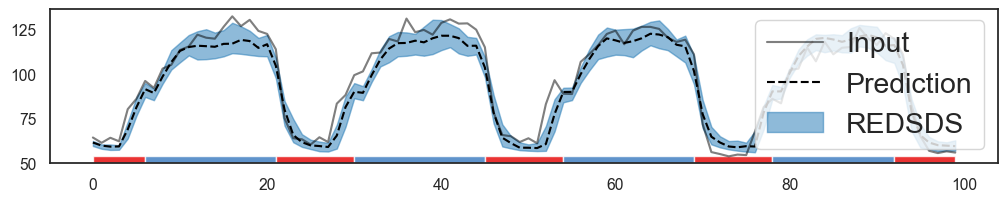
\includegraphics[width=0.49\linewidth]{changepoints/figs/e-prob.png}
    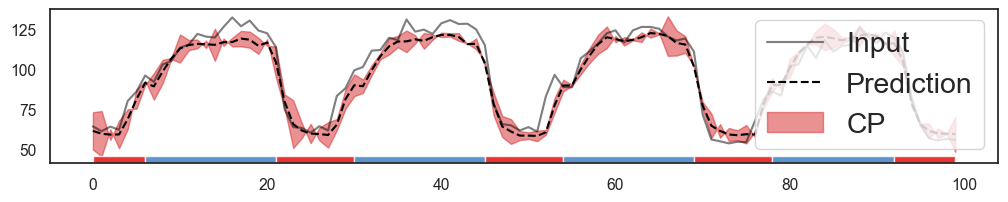
\includegraphics[width=0.49\linewidth]{changepoints/figs/e-cp.png}
    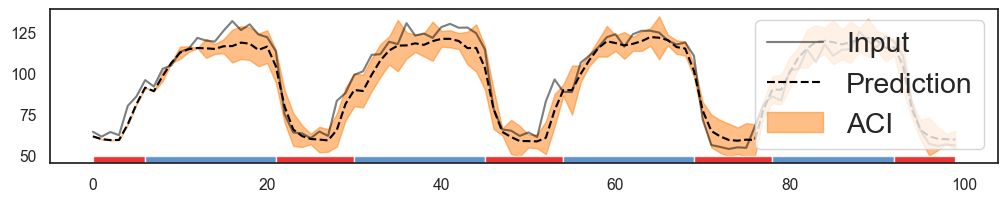
\includegraphics[width=0.49\linewidth]{changepoints/figs/e-aci.png}
    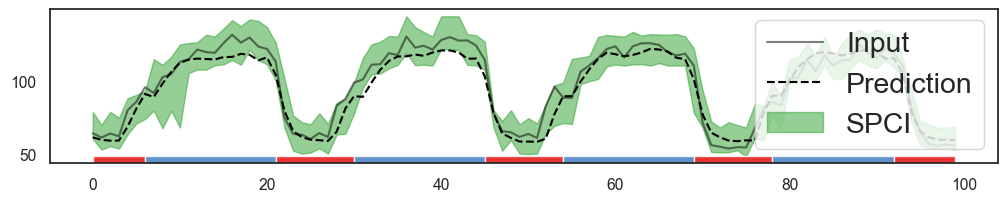
\includegraphics[width=0.49\linewidth]{changepoints/figs/e-spci.png}
    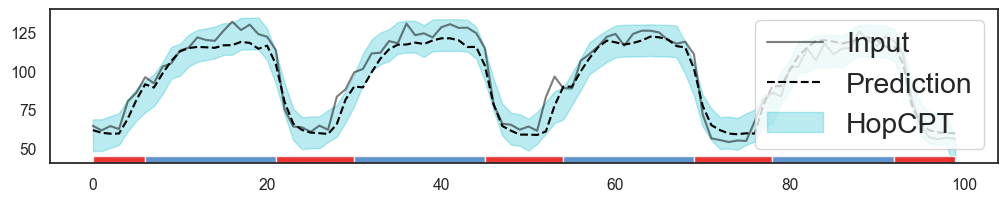
\includegraphics[width=0.49\linewidth]{changepoints/figs/e-hop.png}
    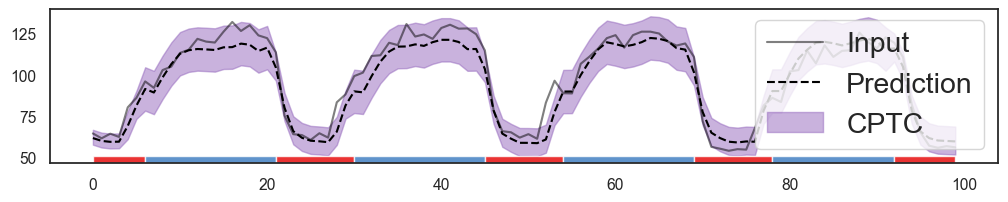
\includegraphics[width=0.49\linewidth]{changepoints/figs/e-ours.png}
    \vspace{-0.5em}
    \caption{\textbf{Visualization of prediction intervals on the Electricity hourly demand dataset.} The red and blue bars in the bottom reflects the underlying switching state of day and night. Our method (purple) adapts to different levels of volatility between day and night, and achieves stabler coverage over time, whereas ACI (yellow) over-covers during the night and under-covers at change points.}
    \label{fig:demonstration}
\vspace{-1em}
\end{figure}


 
%\sofi{Some more visualizations}
%\subsection{Ablation study on aggreagation methods} 
%\sofi{Ablation study on aggreagation methods, ablation on sequence length?}

\vspace{-0.6em}
\subsection{Ablation Studies}
\label{sec:accuracy}
\vspace{-0.5em}
\paragraph{Robustness to $p(\hat{z})$ accuracy.} We conduct ablation studies on the 3 synthetic datasets of which we have ground truth underlying states. As shown in table \ref{tab:z_exp}, it is evident that increasing the error in the state prediction does not affect the coverage performance. This verifies the robustness of our algorithm and theoretical results (Theorem \ref{thm:asymptotic_validity} and \ref{thm:imperfect_state_predictions}). Table \ref{tab:z_exp_area} further shows that the error of state prediction reflects on the width of the prediction intervals: while remaining the same level of coverage, the better the state predictions, the sharper the intervals.

\vspace{-1.5em}
\begin{minipage}{0.58\textwidth}
\begin{table}[H]
    \caption{Coverage of CPTC for using ground truth (GT) labels and with various levels of injected noise, on synthetic data with $T=200$. We can see that coverage performance does not change significantly with error in state prediction. }   
    \vspace{0.4em}
    \label{tab:z_exp}
    \centering
    \resizebox{\textwidth}{!}{%
    \begin{tabular}{c|c c c}
        \toprule
        & Ground truth state labels & GT w/ $20\%$ error & GT w/ $50\%$ error \\ 
        \midrule
        BB obs.  & 90.31 \plusminus 1.27 & 90.27 \plusminus 1.30 & 90.13 \plusminus 1.40 \\ 
        BB dyn.  & 90.34 \plusminus 0.93 & 90.32 \plusminus 0.96 & 90.33 \plusminus 1.05 \\ 
        3-mode  & 92.67 \plusminus 1.52 &  92.70 \plusminus 1.63  & 92.53 \plusminus 1.54 \\ 
        \bottomrule
    \end{tabular}
    }
\end{table}

\end{minipage}
\hfill
\begin{minipage}{0.38\textwidth}
\begin{table}[H]
    \centering
    \caption{Interval width under the same setting. While the coverage guarantee is the same, the more accurate the state prediction is, the sharper the intervals.}
    \vspace{0.4em}
    \label{tab:z_exp_area}
    \resizebox{\textwidth}{!}{%
    \begin{tabular}{c| c c c}
        \toprule
        & GT & w/ $20\%$ err & w/ $50\%$ err\\ 
        \midrule
        BB obs. & 3.61 \plusminus 0.93 & 3.75 \plusminus 0.99 & 3.94 \plusminus 1.17 \\ 
        BB dyn. & 2.09 \plusminus 0.60 & 2.15 \plusminus 0.62 & 2.18 \plusminus 0.65 \\ 
        3-mode & 2.04 \plusminus 0.67 &  2.19 \plusminus 0.76  & 2.27 \plusminus 0.89 \\ 
        \bottomrule
    \end{tabular}
    }       
\end{table}
\end{minipage}

\vspace{0.5em}
Additional ablation studies are presented in Appendix \ref{app:more_experiments}. On \textbf{Aggregation Methods} (by discretization as \Eqref{eq:aggregation-average} or union as \Eqref{eq:aggregation-union}), we found that on our benchmark datasets, union is a close proximation of the true objective, and CPTC achieves similar width and coverage on a sampled subset. For \textbf{Long Horizon Forecasting} where $T \geq 10,000$, our method still achieves valid and stable coverage, but have wider PI width compared to SPCI an HopCPT. They achieve this by frequently re-training their models online, which CPTC does not and is less computationally demanding.